
\begin{enumerate}
\item There is a junction in a circuit that has one wire with current flowing in and two wires with current flowing out.  There is $1.25\myamp$ of current coming in, and the first wire going out has $0.15\myamp$ of current going out.  How much current is leaving through the second wire?
\item There is a junction in a circuit that has two wires with current flowing in and two wires with current flowing out.  The first wire with current flowing in has $0.35\myamp$ of current, the first wire with current flowing out has $0.25\myamp$ of current, and the second wire with current flowing out has $0.42\myamp$ of current.  How much current is flowing in on the second incoming wire?
\item At a junction of four wires, wire 1 has $0.1\myamp$ of current flowing in, wire 2 has $0.2\myamp$ of current flowing in, and wire 3 has $0.4\myamp$ of current flowing out.  Is the current in wire 4 going in or out?  How much current is flowing on it?
\item If I have three $100\myohm$ resistors in series, what is the total resistance of the series?
\item If I have a $10\myohm$ resistor, a $30\myohm$ resistor, and a $65\myohm$ resistor in series, what is the total resistance of the series?
\item If I have a $5\myohm$ resistor and a $7\myohm$ resistor in series, what is the total resistance of the series?
\item If I have two resistors in parallel, a $30\myohm$ resistor and a $40\myohm$ resistor, what is the total resistance of this circuit?
\item If I have three resistors in parallel---$25\myohm$, $40\myohm$, and $75\myohm$, what is the total resistance of this circuit?
\item If I have four resistors in parallel---$1,000\myohm$, $800\myohm$, $2,000\myohm$, and $5,000\myohm$, what is the total resistance of this circuit?
\item If I have three resistors in parallel---$100\myohm$, $5,000\myohm$, and $10,000\myohm$---what is the total resistance of this circuit?  Which of the resistors is the total resistance most similar to?
\item Take a look at the following circuit diagram.  If the voltage drop between B and C is 2 volts, and the voltage drop between C and D is 3 volts, what is the voltage drop between A and E?  What is the voltage at E?  What is the voltage at A? \\ 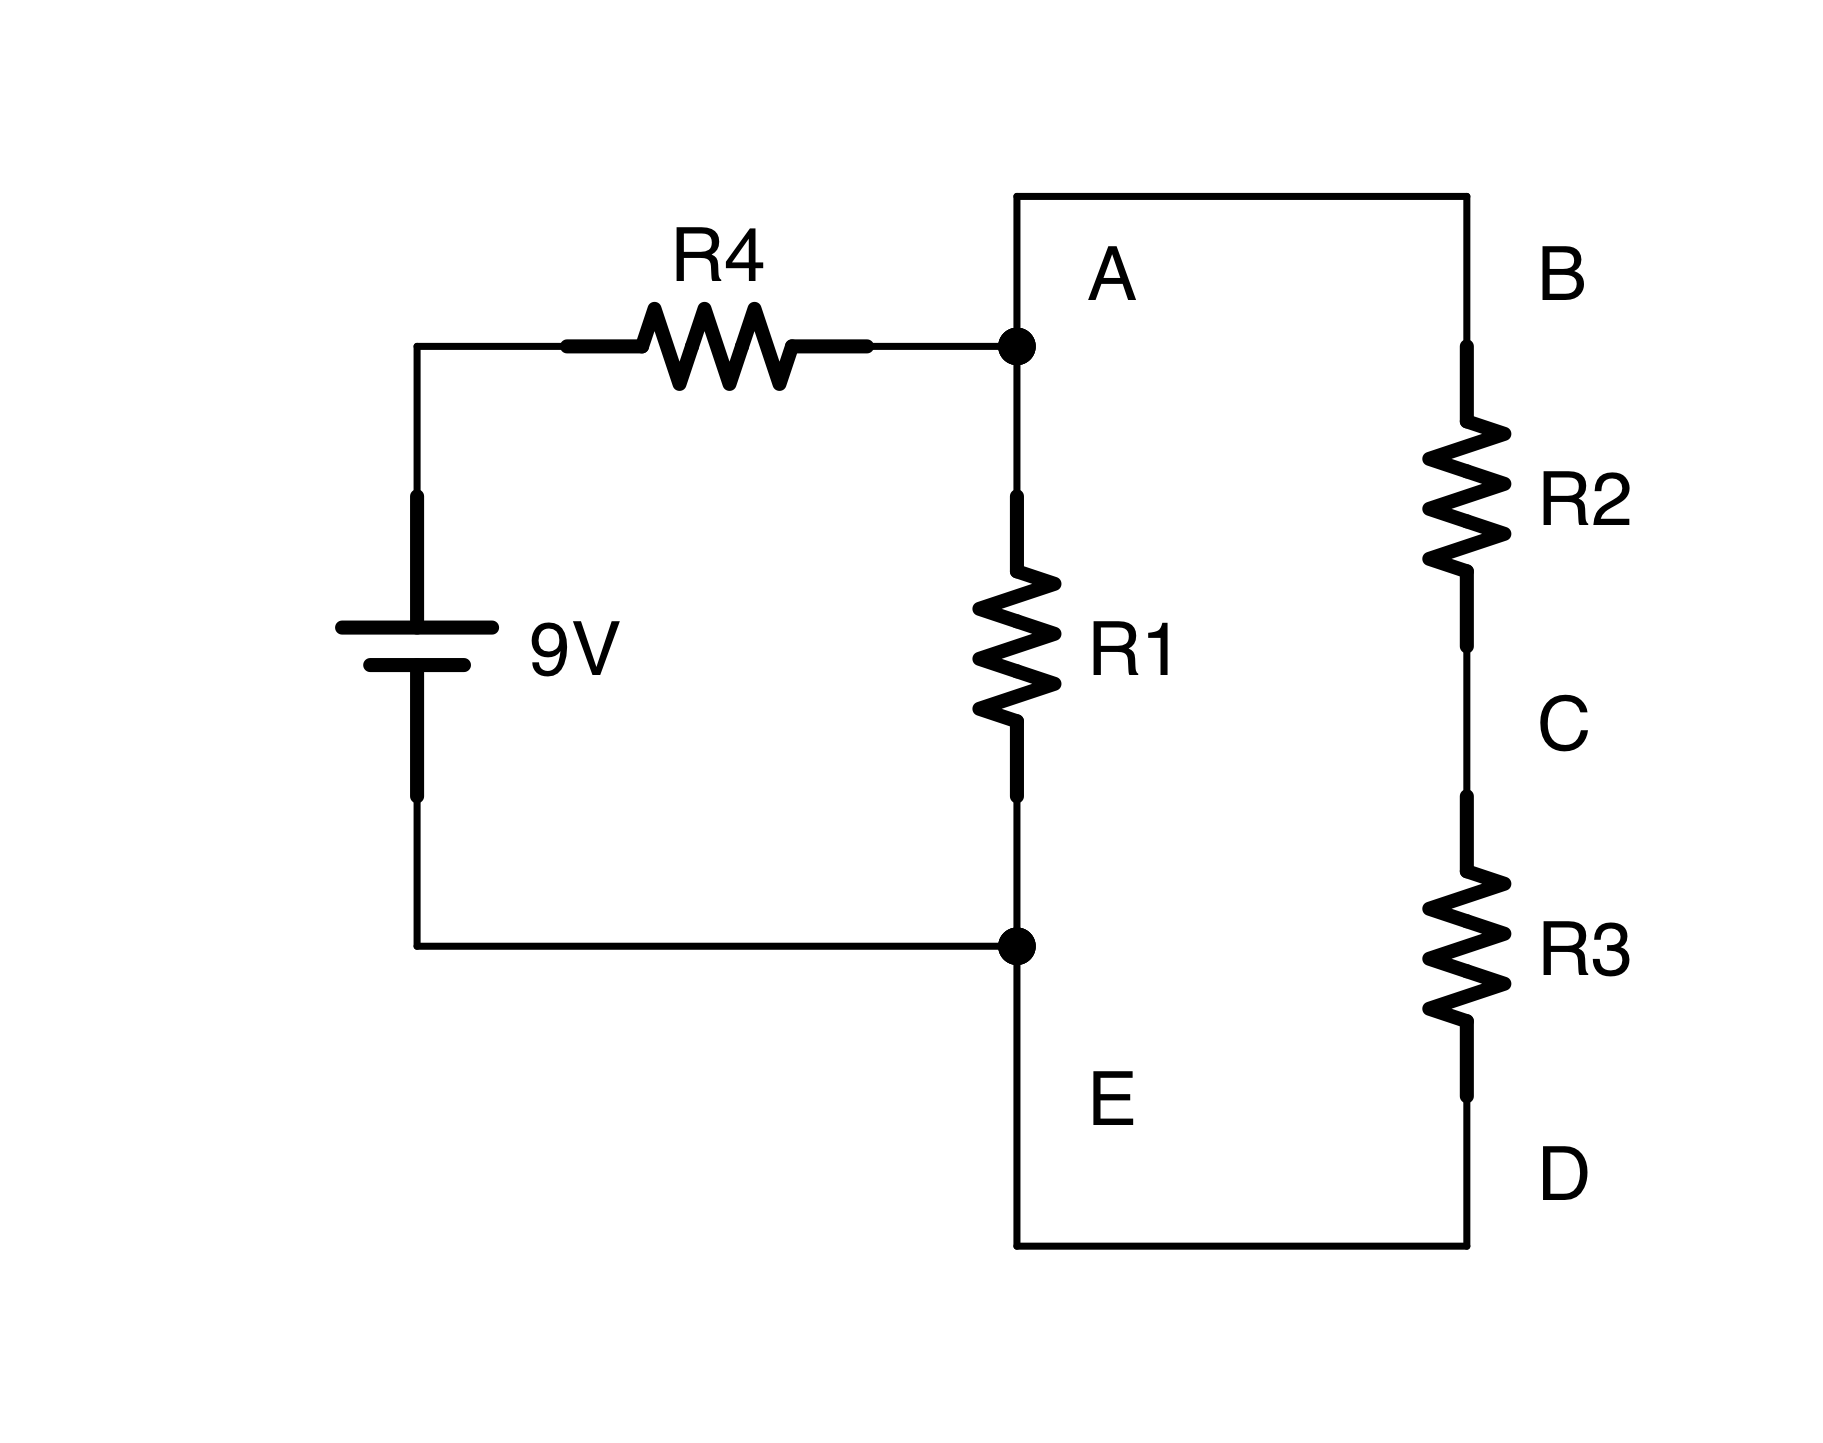
\includegraphics[scale=0.08]{VoltageDropProblem.png}
\item Optional - what resistor values would you need to have the circuit above run with $2\myamp$ total current?
\item The circuit below is a combination of series and parallel resistances.  Each resistor is labelled with its resistance value, given in ohms.  Find out how much current is flowing through each resistor, and how much each resistor drops the voltage.  \\ 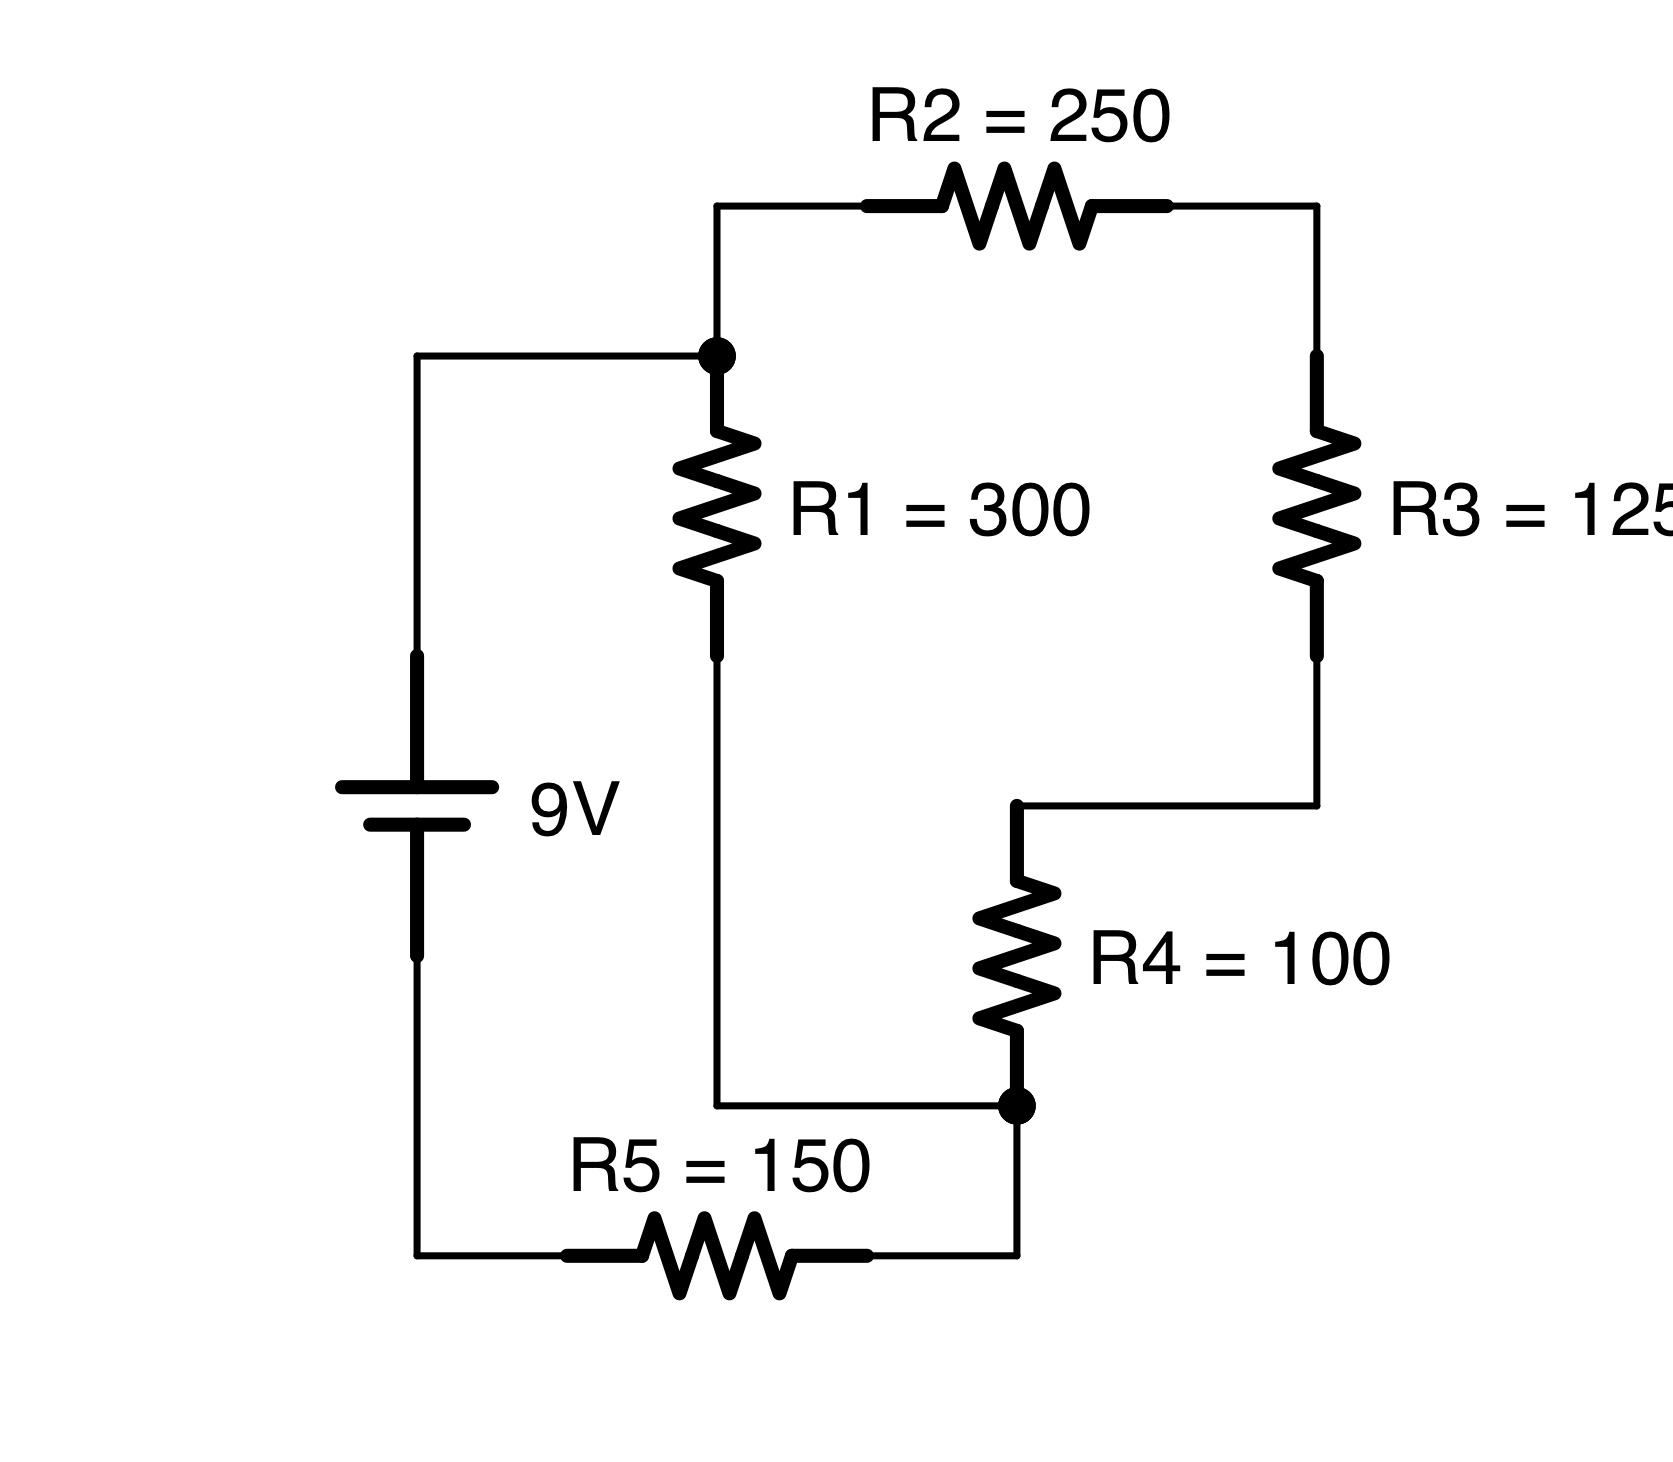
\includegraphics[scale=0.08]{ProblemCalculateCurrentAndVoltage.png}
\item Build the circuit in Figure~\ref{figParallelUsingBreadboard} on your own breadboard.  Measure the voltage drops across every component, and measure the amount of current flowing into the first series resistor.
\end{enumerate}
